% Shared section: used by paper-ieee.tex, paper-lncs.tex and report.tex.
% Use \sect / \subsect for headings (see README), never \section directly.

\sect{Results}\label{results}

\iffull
\subsect{Later hand-labelled development artifact}\label{later-hand-labelled-development-artifact}
\fi

\iffull
The hand-labelled model is \nolinkurl{pinch_in-ae0a22bf}, SHA-256 \nolinkurl{ae0a22bf8f744d5fa2fce9208221f0947288c5ba5c5eb196180985a70d77ba0d}. Its bytes match the manifest, as do those of all seven model files in the project. This confirms the files are intact; it does not tell us which model is running on any given laptop.
\else
We evaluate the hand-labelled pinch-in model \nolinkurl{pinch_in-ae0a22bf}, whose file matches its declared SHA-256. Its threshold was chosen on the training recordings, not on the evaluation set, and its stored window ROC AUC is 0.982.
\fi

\iffull
The manifest records a window ROC AUC of 0.981993, balanced accuracy of 0.881720 and window F1 of 0.865854, together with an event recall of 0.824561 and no false activations. The threshold was chosen on the training recordings (\nolinkurl{thresholdChosenOnEvaluationRecordings} is false). That is a stronger separation than tuning on the evaluation set, but the evaluation recordings may still have influenced label edits, architecture choices or which candidate model was kept.
\fi

\iffull
\begin{table}[t]
\centering\small
\caption[Stored manifest fields of the pinch-in model]{Stored manifest fields for the pinch-in model. The event values were reproduced by replay. These are development results, not a prospective test.}
\begin{tabularx}{\linewidth}{@{}>{\raggedright\arraybackslash}Xr>{\raggedright\arraybackslash}X@{}}
\toprule
\textbf{Field} & \textbf{Value} & \textbf{Status} \\
\midrule
Training IDs & 20 & All resolved \\
Evaluation IDs & 8 & All resolved \\
Event recall & 82.46\% (47/57) & Reproduced \\
False activations & 0 in 0.48 h & Reproduced \\
Window ROC AUC & 0.981993 & Window-level \\
Window F1 & 0.865854 & Window-level \\
\bottomrule
\end{tabularx}
\end{table}
\fi

\iffull
The model was saved without its event log, so we recovered it by replay. The exact training specification was not saved either. We rebuilt the label roles from the project's documented defaults and tried all four combinations of the two uncertain settings (whether \nolinkurl{left_out} is excluded, and whether the still-hand rule applies); all four gave the same result. Running the stored model over the eight evaluation recordings with the trainer's own input building, detection rule and event accounting reproduced the stored metrics exactly (Table~\ref{tab-replay}).
\else
The model was saved without its event log, so we recovered it by replaying the stored model over its eight evaluation recordings with the trainer's own code. This reproduced the stored metrics exactly (Table~\ref{tab-replay}).
\fi

\begin{table}[t]
\centering\small
\caption[Replayed event outcomes of the pinch-in model]{Replayed event outcomes of the hand-labelled pinch-in model on its eight evaluation recordings.}\label{tab-replay}
\begin{tabularx}{\linewidth}{@{}>{\raggedright\arraybackslash}Xr>{\raggedright\arraybackslash}X@{}}
\toprule
\textbf{Outcome} & \textbf{Value} & \textbf{Basis} \\
\midrule
Caught / eligible starts & 47 / 57 (82.5\%) & Matches manifest \\
By day (3, 4, 6 Nov) & 17/18, 17/21, 13/18 & Replay \\
Missed & 10 (4 late, 6 undetected) & Replay \\
Repeats; false activations & 0; 0 & Matches manifest \\
Eligible no-gesture time & 1,735.4 s (0.48 h) & Replay, no gaps \\
95\% upper false-activation rate & 6.2 per hour & Poisson, zero events \\
Latency, median (IQR; p95) & 442 ms (384--510; 649) & From emission \\
\bottomrule
\end{tabularx}
\end{table}

\iffull
Figure~\ref{fig:score-timeline} shows how this looks over time for one evaluation recording, the pinch-hold session of 4 November. Of its 21 annotated starts, 17 were caught. The other four show three different ways a pinch can be missed. One produced no response at all. One raised the score to 0.906, short of the 0.99 activation threshold. The remaining two produced an event about 280\,ms after the start, just before the 300\,ms match window opens; the evaluation counts these as late, although they came slightly early. Between pinches the score stays close to zero, and the recording has no false activations. Figure~\ref{fig:latency} shows the latencies of all 47 caught starts across the eight recordings: most fall between 350 and 550\,ms, with a tail up to 755\,ms.

\begin{figure}[htbp]
\centering
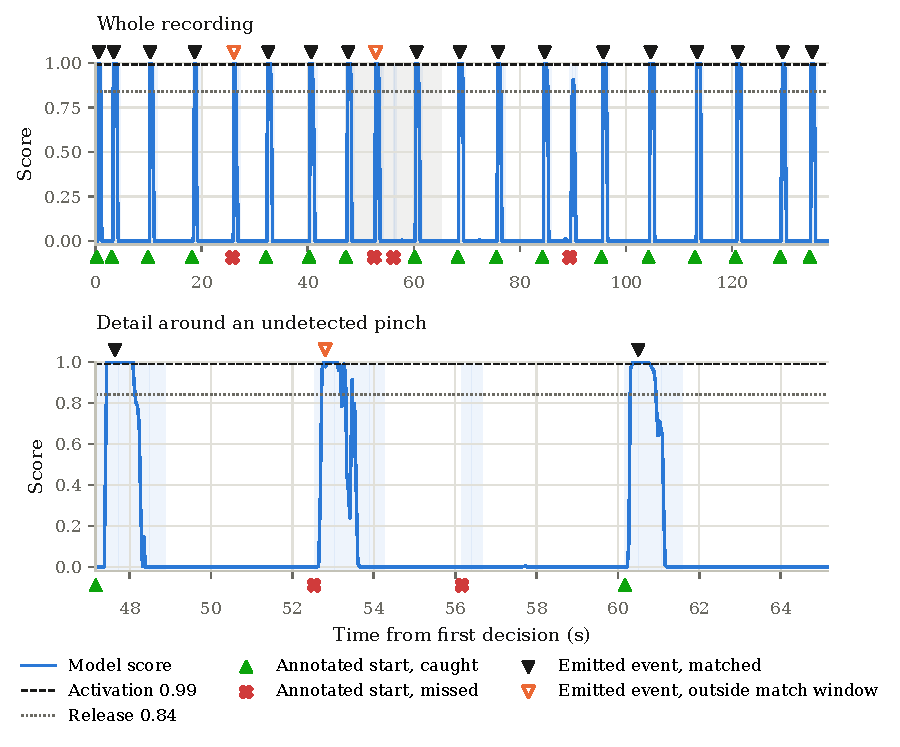
\includegraphics[width=\linewidth]{figures/score-timeline.pdf}
\caption[Model score over an evaluation recording]{Score of the hand-labelled pinch-in model over the evaluation recording \nolinkurl{gesture-dataset-pinch_hold-2026-11-04T04-50-33.518Z}, replayed with the trainer's own detection rule. Shaded bands are annotated pinch gestures; markers below the axis are annotated starts, markers above are emitted events. The grey region in the top panel is shown in detail below.}\label{fig:score-timeline}
\end{figure}

\begin{figure}[htbp]
\centering
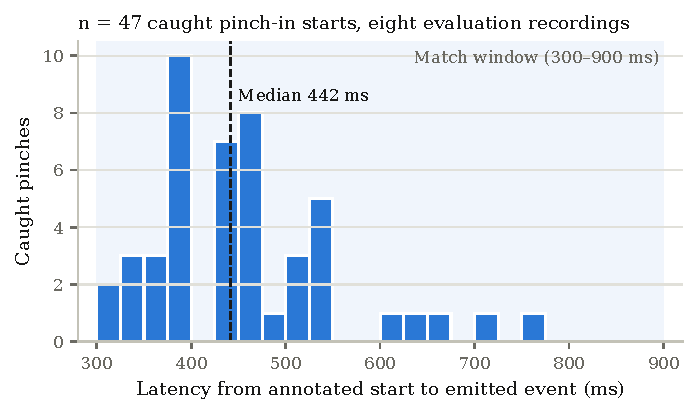
\includegraphics[width=0.85\linewidth]{figures/latency-histogram.pdf}
\caption[Latency of caught pinches]{Latency from the annotated start to the emitted event for the 47 caught pinch-in starts in the eight evaluation recordings (25\,ms bins). The shaded region is the 300--900\,ms match window.}\label{fig:latency}
\end{figure}
\fi

\iffull
Latency is measured from the annotated start to the moment the event is emitted. The margin behind the zero false-activation count is thin. In the everyday-activity recording the highest score reached 0.970, just under the 0.99 threshold; lowering the threshold to 0.98 would have added one false activation, and 0.95 would have added two. We report this as a sensitivity check, not as a reason to pick a different threshold.
\else
The margin behind the zero false-activation count is thin. In the everyday-activity recording the highest score reached 0.970 against the 0.99 threshold, and thresholds of 0.98 and 0.95 would have added one and two false activations.
\fi

\iffull
There is no hand-labelled pinch-out model. A median pinch-out model exists, but its training data cannot be traced, so it is not a matched counterpart. The result above therefore covers pinch-in only, not the full grab-and-release interaction.
\else
There is no matched hand-labelled pinch-out model, so these results cover pinch-in only.
\fi

\iffull
\subsect{Historical camera-label transfer}\label{historical-camera-label-transfer}
\fi

\iffull
The best historical configuration, trained on camera labels with noise recordings and without a still-hand gate and evaluated leave-one-day-out, caught 161 of 372 pinch-in starts (43.3\%). It produced seven false activations per hour on noise recordings and 49 per hour during no-gesture time inside pinch recordings. These rates use different denominators and should not be averaged.
\else
An earlier configuration trained on camera labels caught 161 of 372 pinch-in starts (43.3\%) under leave-one-day-out evaluation, with seven false activations per hour on noise recordings and 49 per hour within pinch recordings. Recall ranged from 21 of 171 on 14 October to 67 of 92 on 3 November (Fig.~\ref{fig-historical}), a spread that a pooled number hides.
\fi

\iffull
Performance varied widely by day: 21 of 171 on 14 October, 37 of 52 on 17 October, 67 of 92 on 3 November and 36 of 57 on 4 November (Fig.~\ref{fig-historical}). The later days support the earlier statement that the model catches about two thirds of unseen pinches; the pooled result does not. An earlier result of 204 of 372 came from a model trained on many October sessions and is not a clean October holdout.
\fi

\begin{widefigure}
\centering
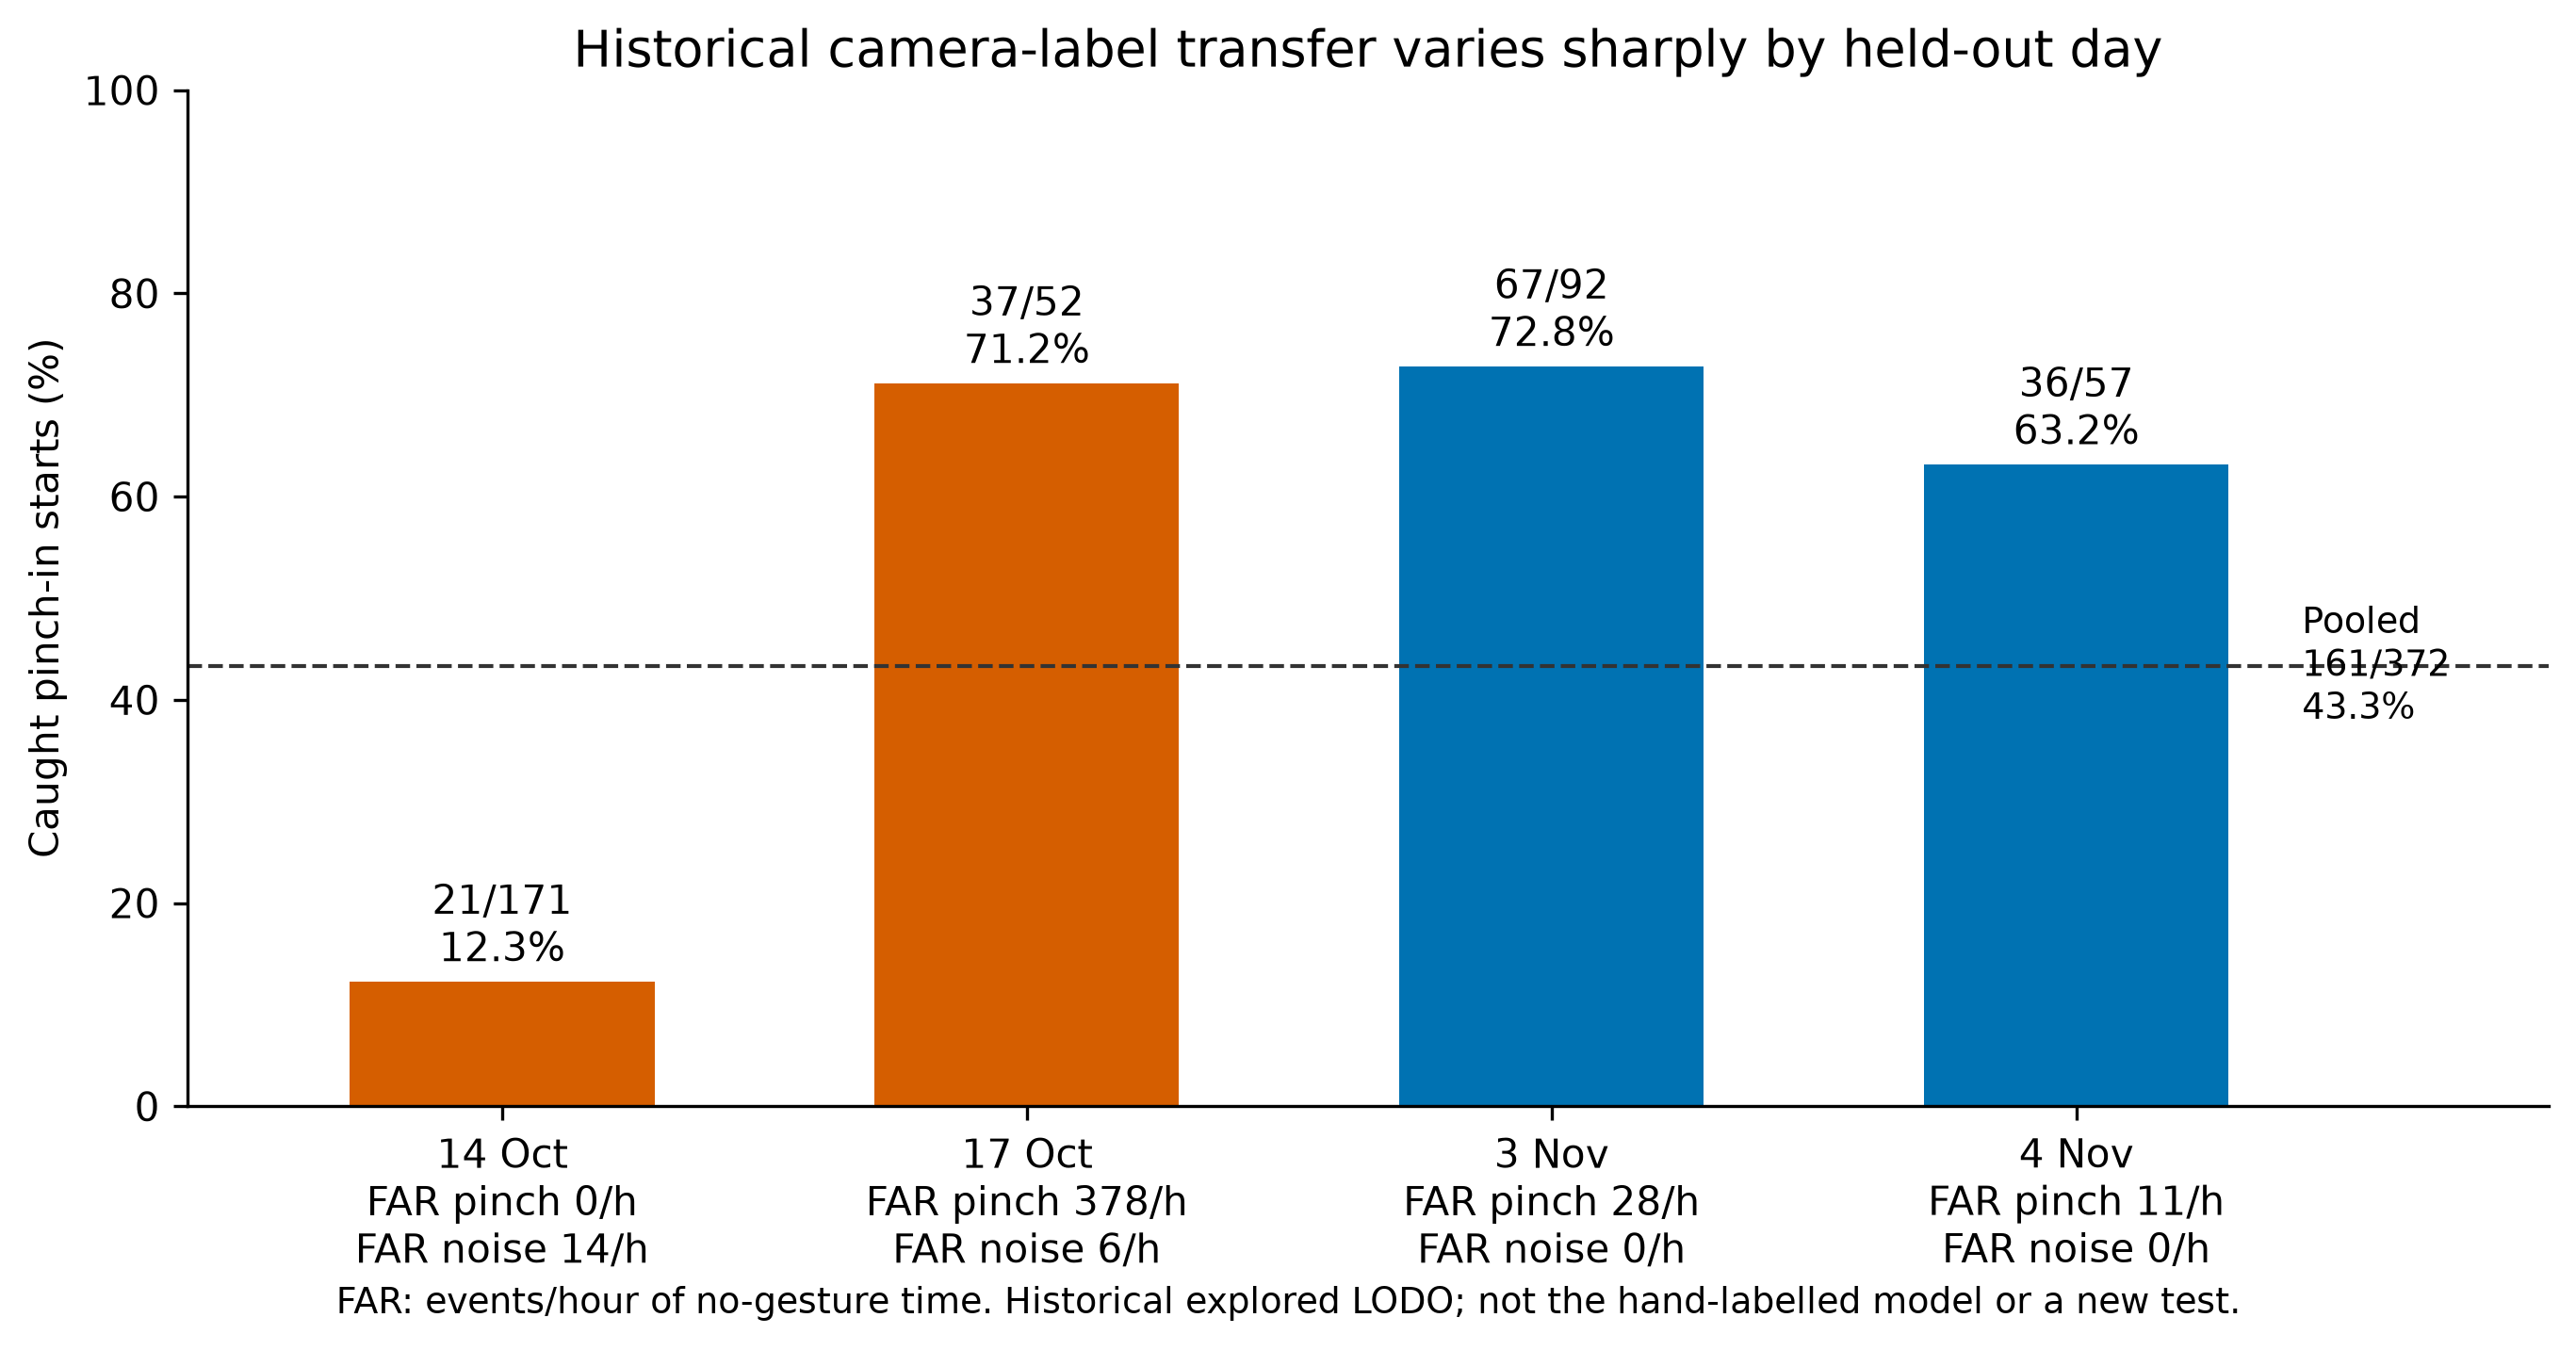
\includegraphics[width=1\linewidth,height=\textheight,keepaspectratio,alt={Historical day-level continuous recall and condition-specific false activations for the selected camera-labelled configuration.}]{figures/historical-day-transfer.png}
\caption[Historical camera-label results by day]{Historical camera-label results, leave-one-day-out. Bars show caught/eligible starts per day; the dashed line is the pooled 161/372. False-activation rates use each condition's own no-gesture time. All days come from one participant.}\label{fig-historical}
\end{widefigure}

\iffull
So, for RQ2: the stored files are intact, the hand-labelled pinch-in split is free of exact duplicates, and the stored development result can be reproduced. We cannot conclude that the manual relabelling improved recall over the older model, because the labels, recordings, preprocessing and thresholds all changed at once.
\else
For RQ2, the stored result is reproducible and its split is free of exact duplicates, but we cannot credit any gain to relabelling, because labels, recordings, preprocessing and thresholds all changed together.
\fi

\iffull
\subsect{Historical diagnostics, not current-model validation}\label{historical-diagnostics-not-current-model-validation}
\fi

\iffull
Earlier fusion experiments on a frozen benchmark raised the worst-split AUC from 0.789 to 0.837. That is a reason to study inertial fusion further, but it does not measure what PPG contributes to the current CNN. A matched comparison of IMU-only, PPG-only and fused inputs is still needed.
\else
Earlier exploratory work points to the open issues behind RQ3. Fusing inertial data raised worst-split AUC from 0.789 to 0.837 on a frozen benchmark, and a strong movement burst can inflate the normalisation scale and hide a pinch that follows it. Both need matched tests on the current model.
\fi

\iffull
The motion-normalisation study found a likely failure mode: a strong movement burst inflates the rolling scale and shrinks a pinch that follows it. Median scaling helped in several synthetic splices, but those numbers only checked whether the peak score 0.1--1\,s after the start crossed the threshold. That is neither continuous causal recall nor a live robustness test, and long bursts were still a problem.
\fi

\iffull
A November curriculum report recorded 15 of 19 pinch-in and 10 of 19 pinch-out catches on a small reserved pair of recordings, with no false activations. The same pair was used to choose the thresholds, so this is exploratory. These results answer RQ3: variation across days, label uncertainty, changes in normalisation and reuse of evaluation data limit our claims more than the choice of architecture does.

\fi